%% QDB Hardware Discussion
\section{The Digital Prototype Design}

This section marks the second part of this chapter.
We describe the design of a digital back-end prototype, which is configured as a 4$\times$4 array of nodes.
Each node is implemented with the logic described in the previous sections.

These nodes are used to test the cotrol logic, communication stability, buffer requirements, and calibration methods.
The most important quantity that much be calibrated for the digital nodes is the frequency of the local oscillator.
The Q-Pix reconstruction for both time and z position are dependent on this parameter, see Chapter~\ref{chap:qpix}.

Since the frequency is the most important quantity, we also dedicate a full section to describe the results of the of local oscillator tests.

Future implementations of the digital back-end for Q-Pix may, of course, use different oscillators.
However, these results are still beneficial as a proof of concept for the frequency calibration, as well as tests to the packet loss susceptibility.
Packet loss is a function of relative frequency drift between neighbor nodes.

\begin{figure}
\centering
\begin{subfigure}{.5\textwidth}
  \centering
  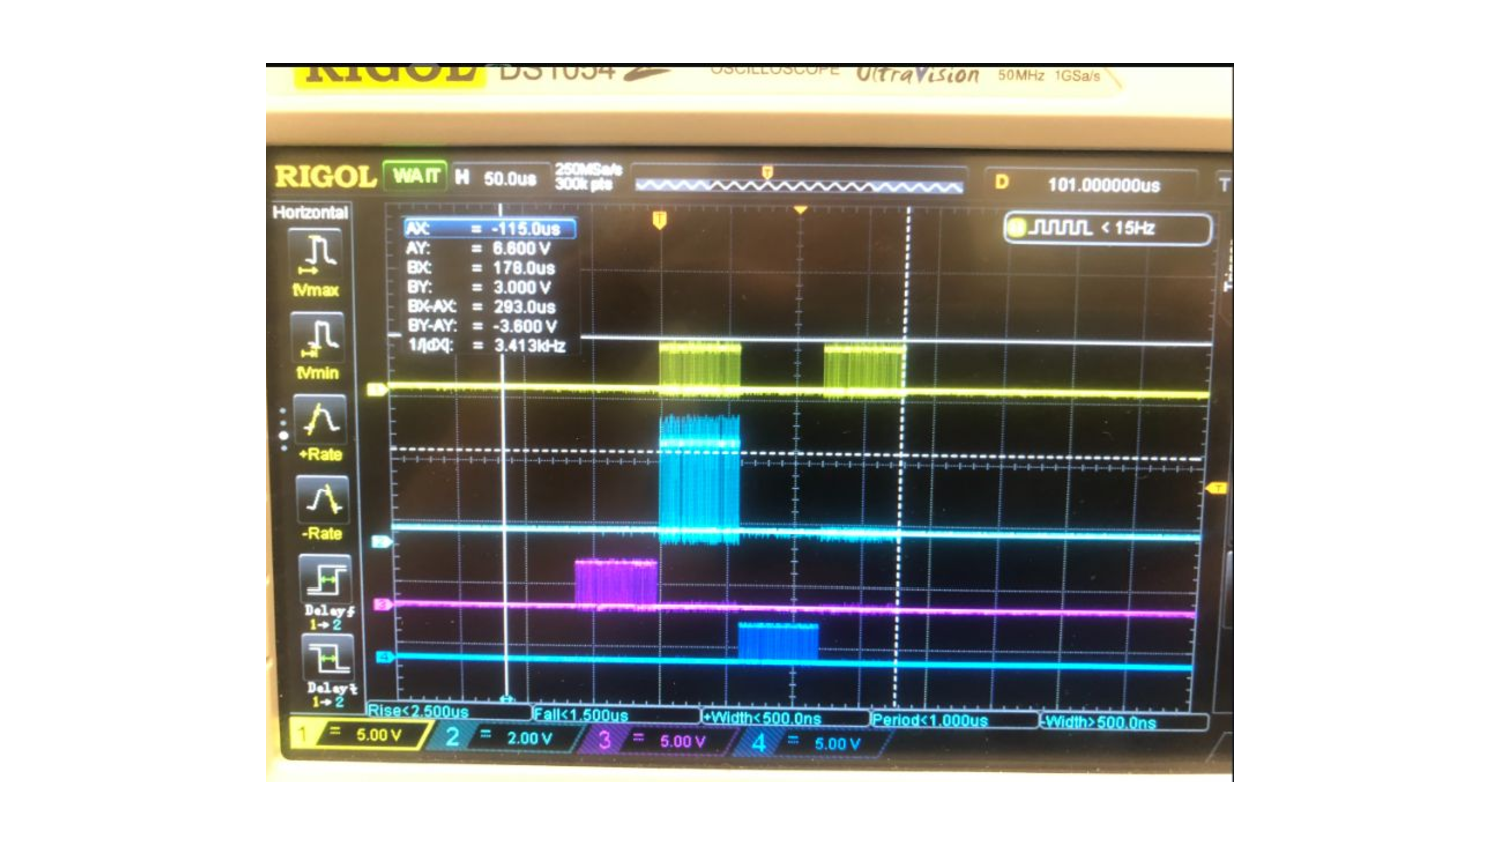
\includegraphics[width=\textwidth]{images/qdb_example_packet_waveform.pdf}
  \caption{Waveforms caught on an oscilloscope. The timescale is 50 $\unit{\mu s}$.}
\end{subfigure}%
\begin{subfigure}{.5\textwidth}
  \centering
  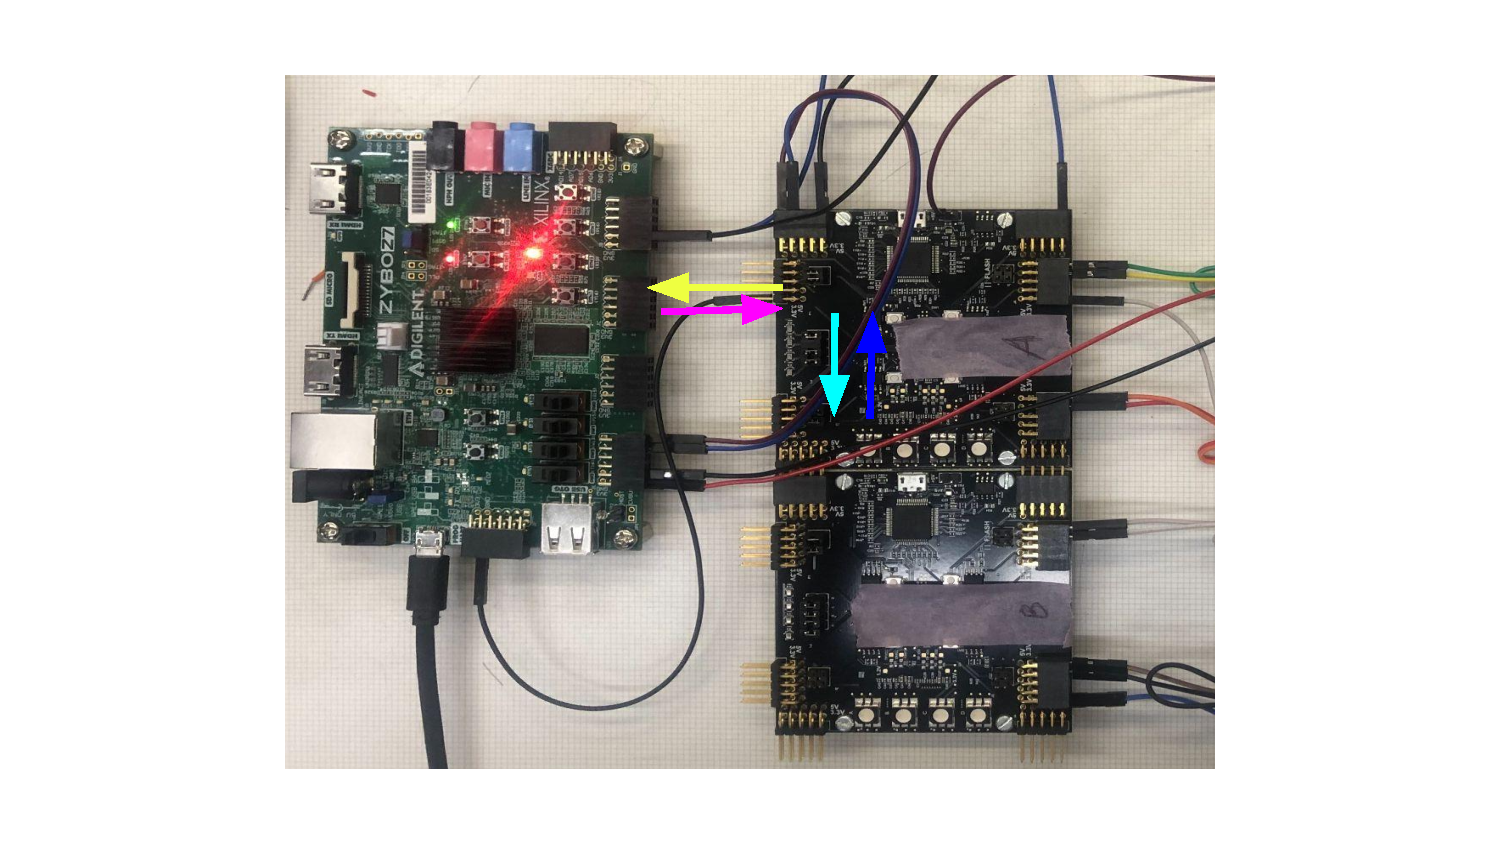
\includegraphics[width=\textwidth]{images/qdb_example_packet_waveform_diagram.pdf}
  \caption{Example of arrows depicting the direction of the packets shown in the other image}
\end{subfigure}
\caption{}
\end{figure}



\subsection{Frequency Calibration of each Node}


%% 4Hz interrogation calibration 
\begin{table}
	\begin{center}
		\begin{tabular}{|c|c|c|c|}
			\hline
			FPGA Position & Mean (30~\unit{MHz}) & STD & $\frac{\delta f}{f_{o}}$*1e6 (ppm) \\
			\hline
			(0,0) & 245.543 & 2.379 & 0.079 \\
			\hline
			(0,1) & 190.646 & 2.979 & 0.099 \\
			\hline
			(0,2) & 153.908 & 3.334 & 0.111 \\
			\hline
			(0,3) & 248.831 & 3.843 & 0.128 \\
			\hline
			(1,0) & 192.729 & 2.860 & 0.095 \\
			\hline
			(1,1) & 210.905 & 3.405 & 0.114 \\
			\hline
			(1,2) & 116.212 & 3.984 & 0.133 \\
			\hline
			(1,3) & 159.824 & 4.158 & 0.139 \\
			\hline
			(2,0) & 351.431 & 3.685 & 0.123 \\
			\hline
			(2,1) & 193.845 & 4.285 & 0.143 \\
			\hline
			(2,2) & 200.278 & 4.071 & 0.136 \\
			\hline
			(2,3) & 152.633 & 4.263 & 0.142 \\
			\hline
			(3,0) & 183.359 & 3.954 & 0.132 \\
			\hline
			(3,1) & 209.788 & 4.561 & 0.152 \\
			\hline
			(3,2) & 192.277 & 4.169 & 0.139 \\
			\hline
			(3,3) & 171.302 & 4.538 & 0.151 \\
			\hline
		\end{tabular}
	\end{center}
	\caption{FPGA calibration results based on Hard Intterrogations at a frequnecy of 4~\unit{Hz}.
	The mean and standard deviation (STD) values are reconstructed for each ASIC within the tile as done in Figure~\ref{fig:frq_recon_node00} and ~\ref{fig:frq_recon_node33}.
	The listed STD value is the result of a gaussian fit performed on the adjusted frequencies.
	}
	\label{tab:fpga_calibration}
\end{table}

\begin{figure}[]
\centering
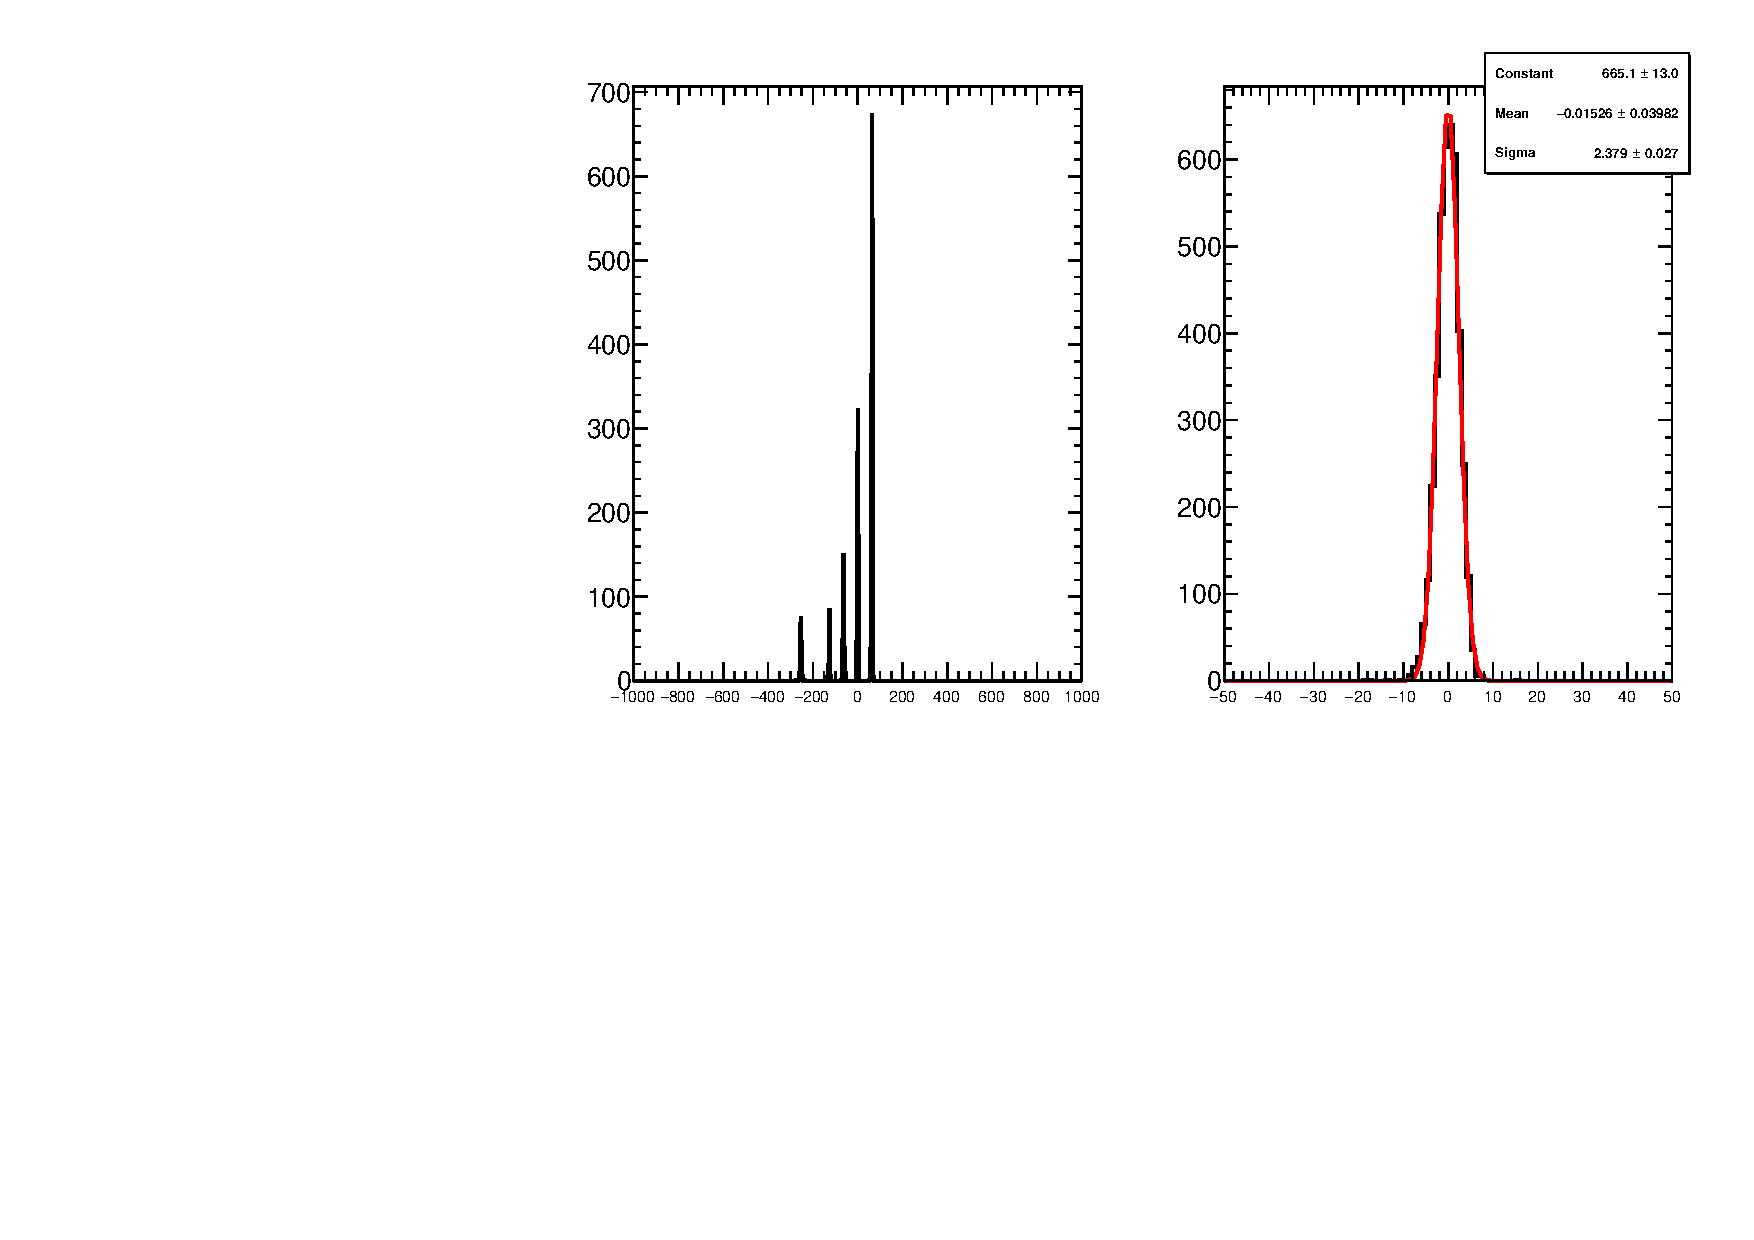
\includegraphics[width=0.5\textwidth]{images/(0,0).pdf}
\caption{Example of frequency calibrations for the FPGA Adjacent to the Zybo.}
\end{figure}

\begin{figure}[]
\centering
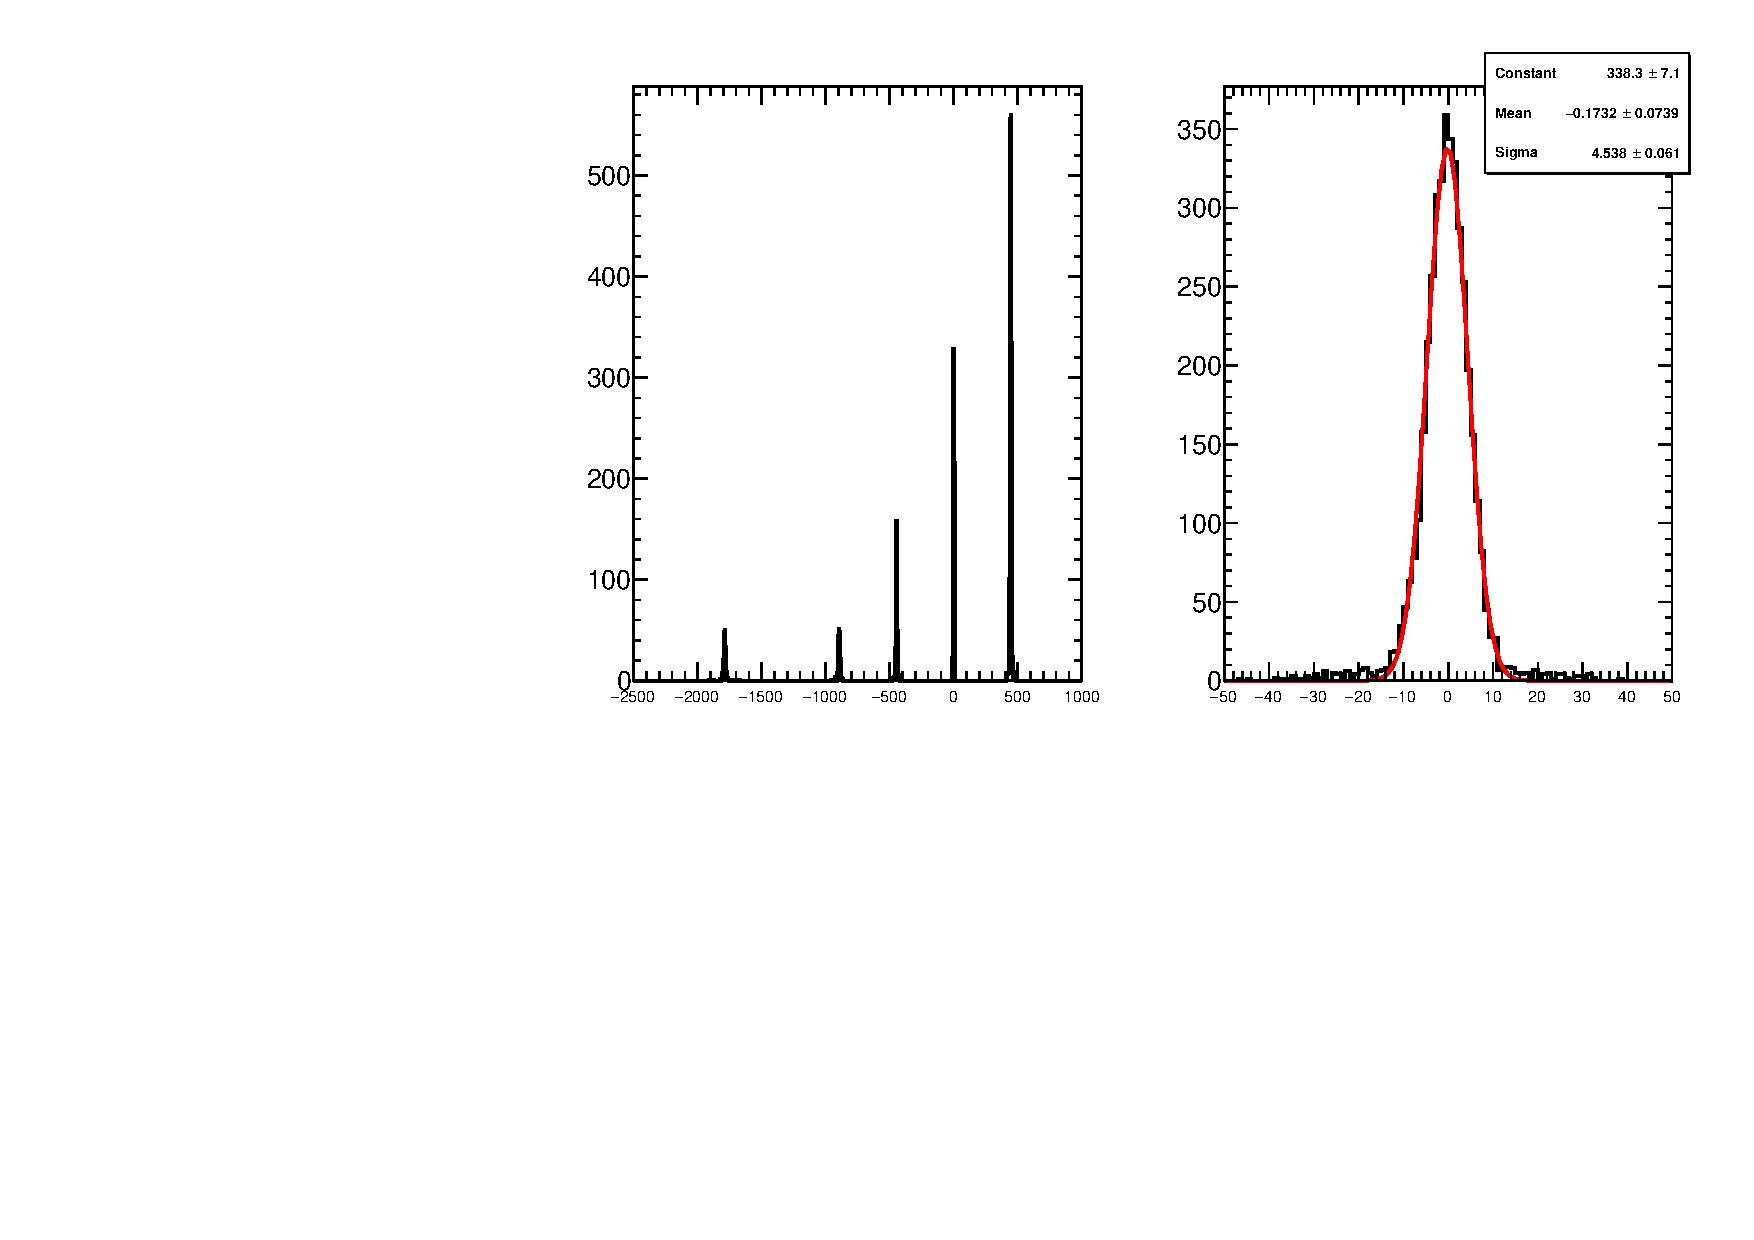
\includegraphics[width=0.5\textwidth]{images/(3,3).pdf}
\caption{}
\end{figure}

\begin{figure}[]
\centering
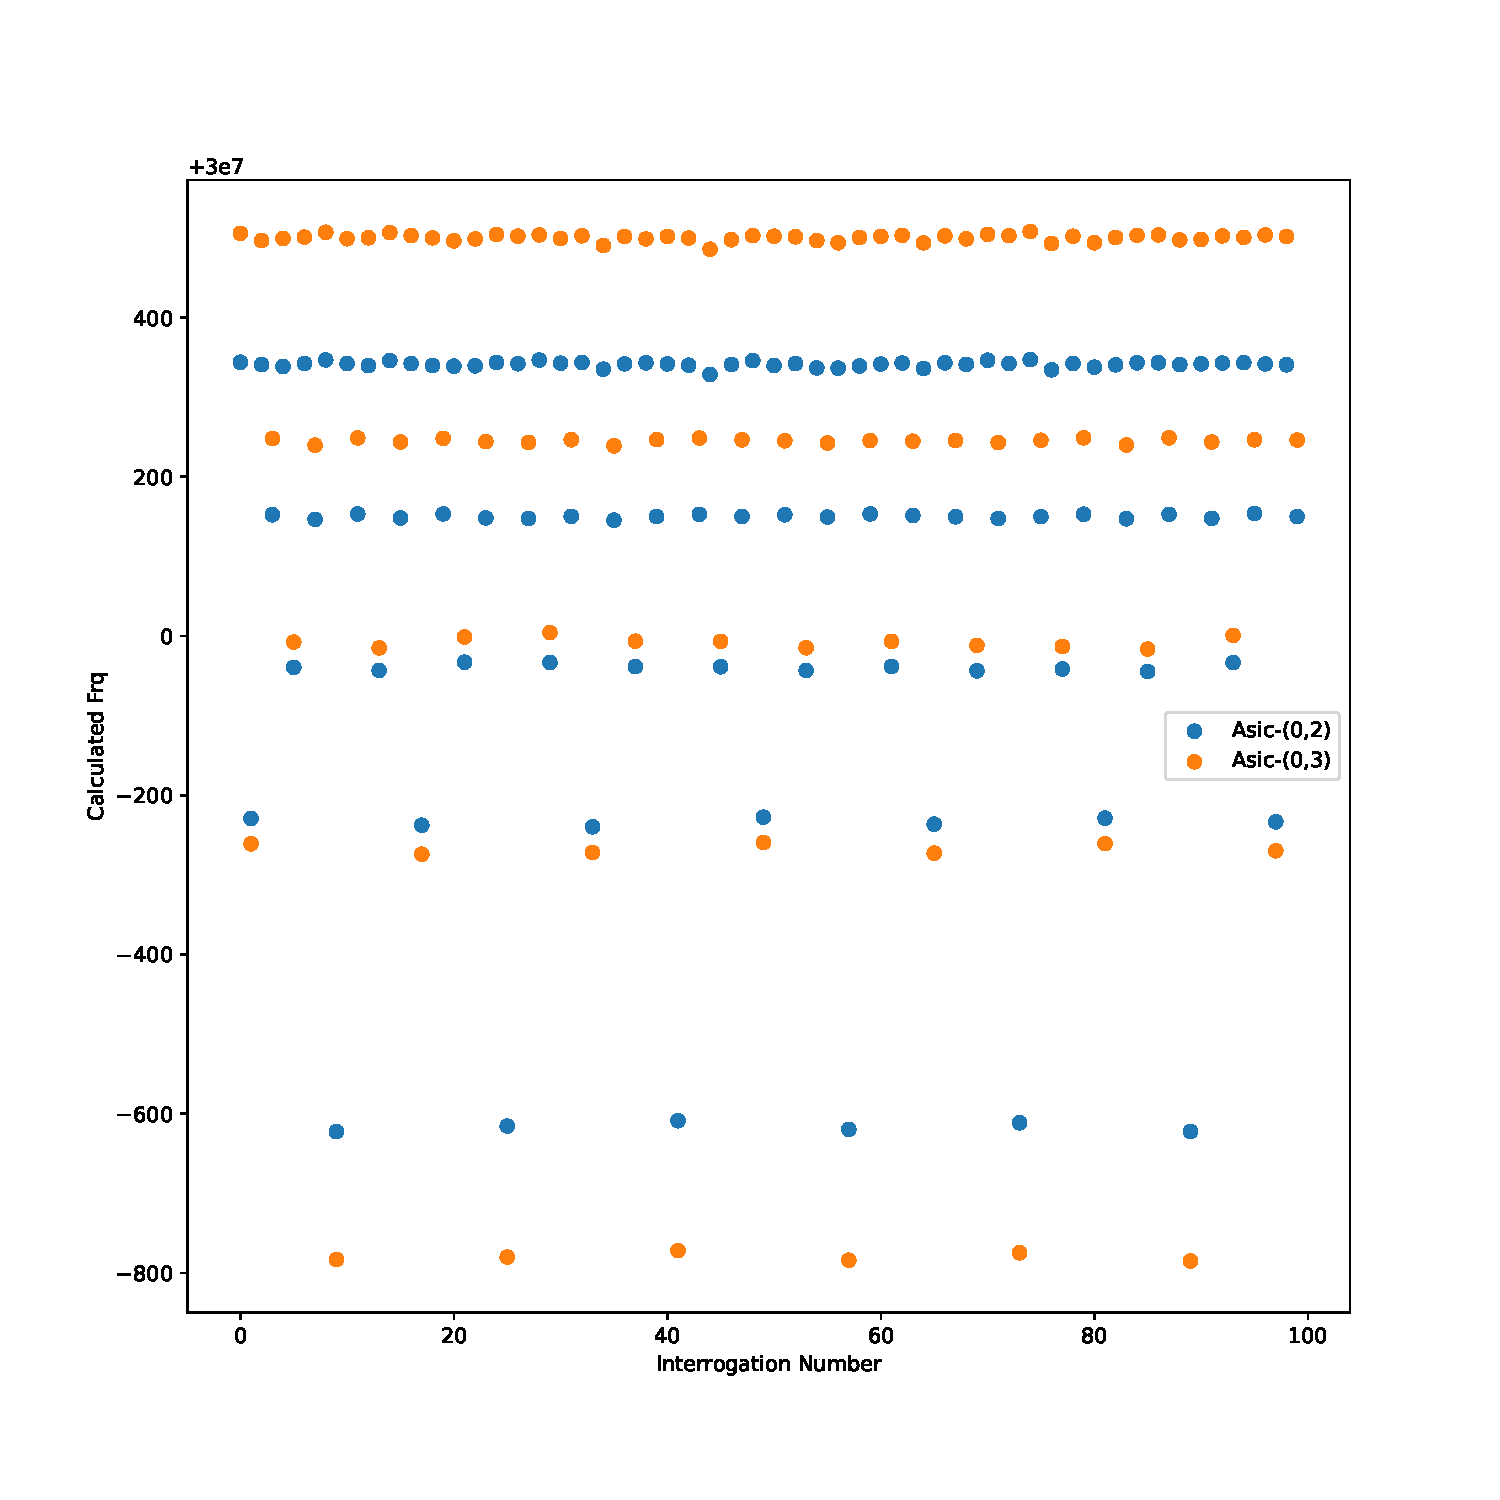
\includegraphics[width=0.5\textwidth]{images/fast_example.pdf}
\caption{}
\end{figure}

\begin{figure}[]
\centering
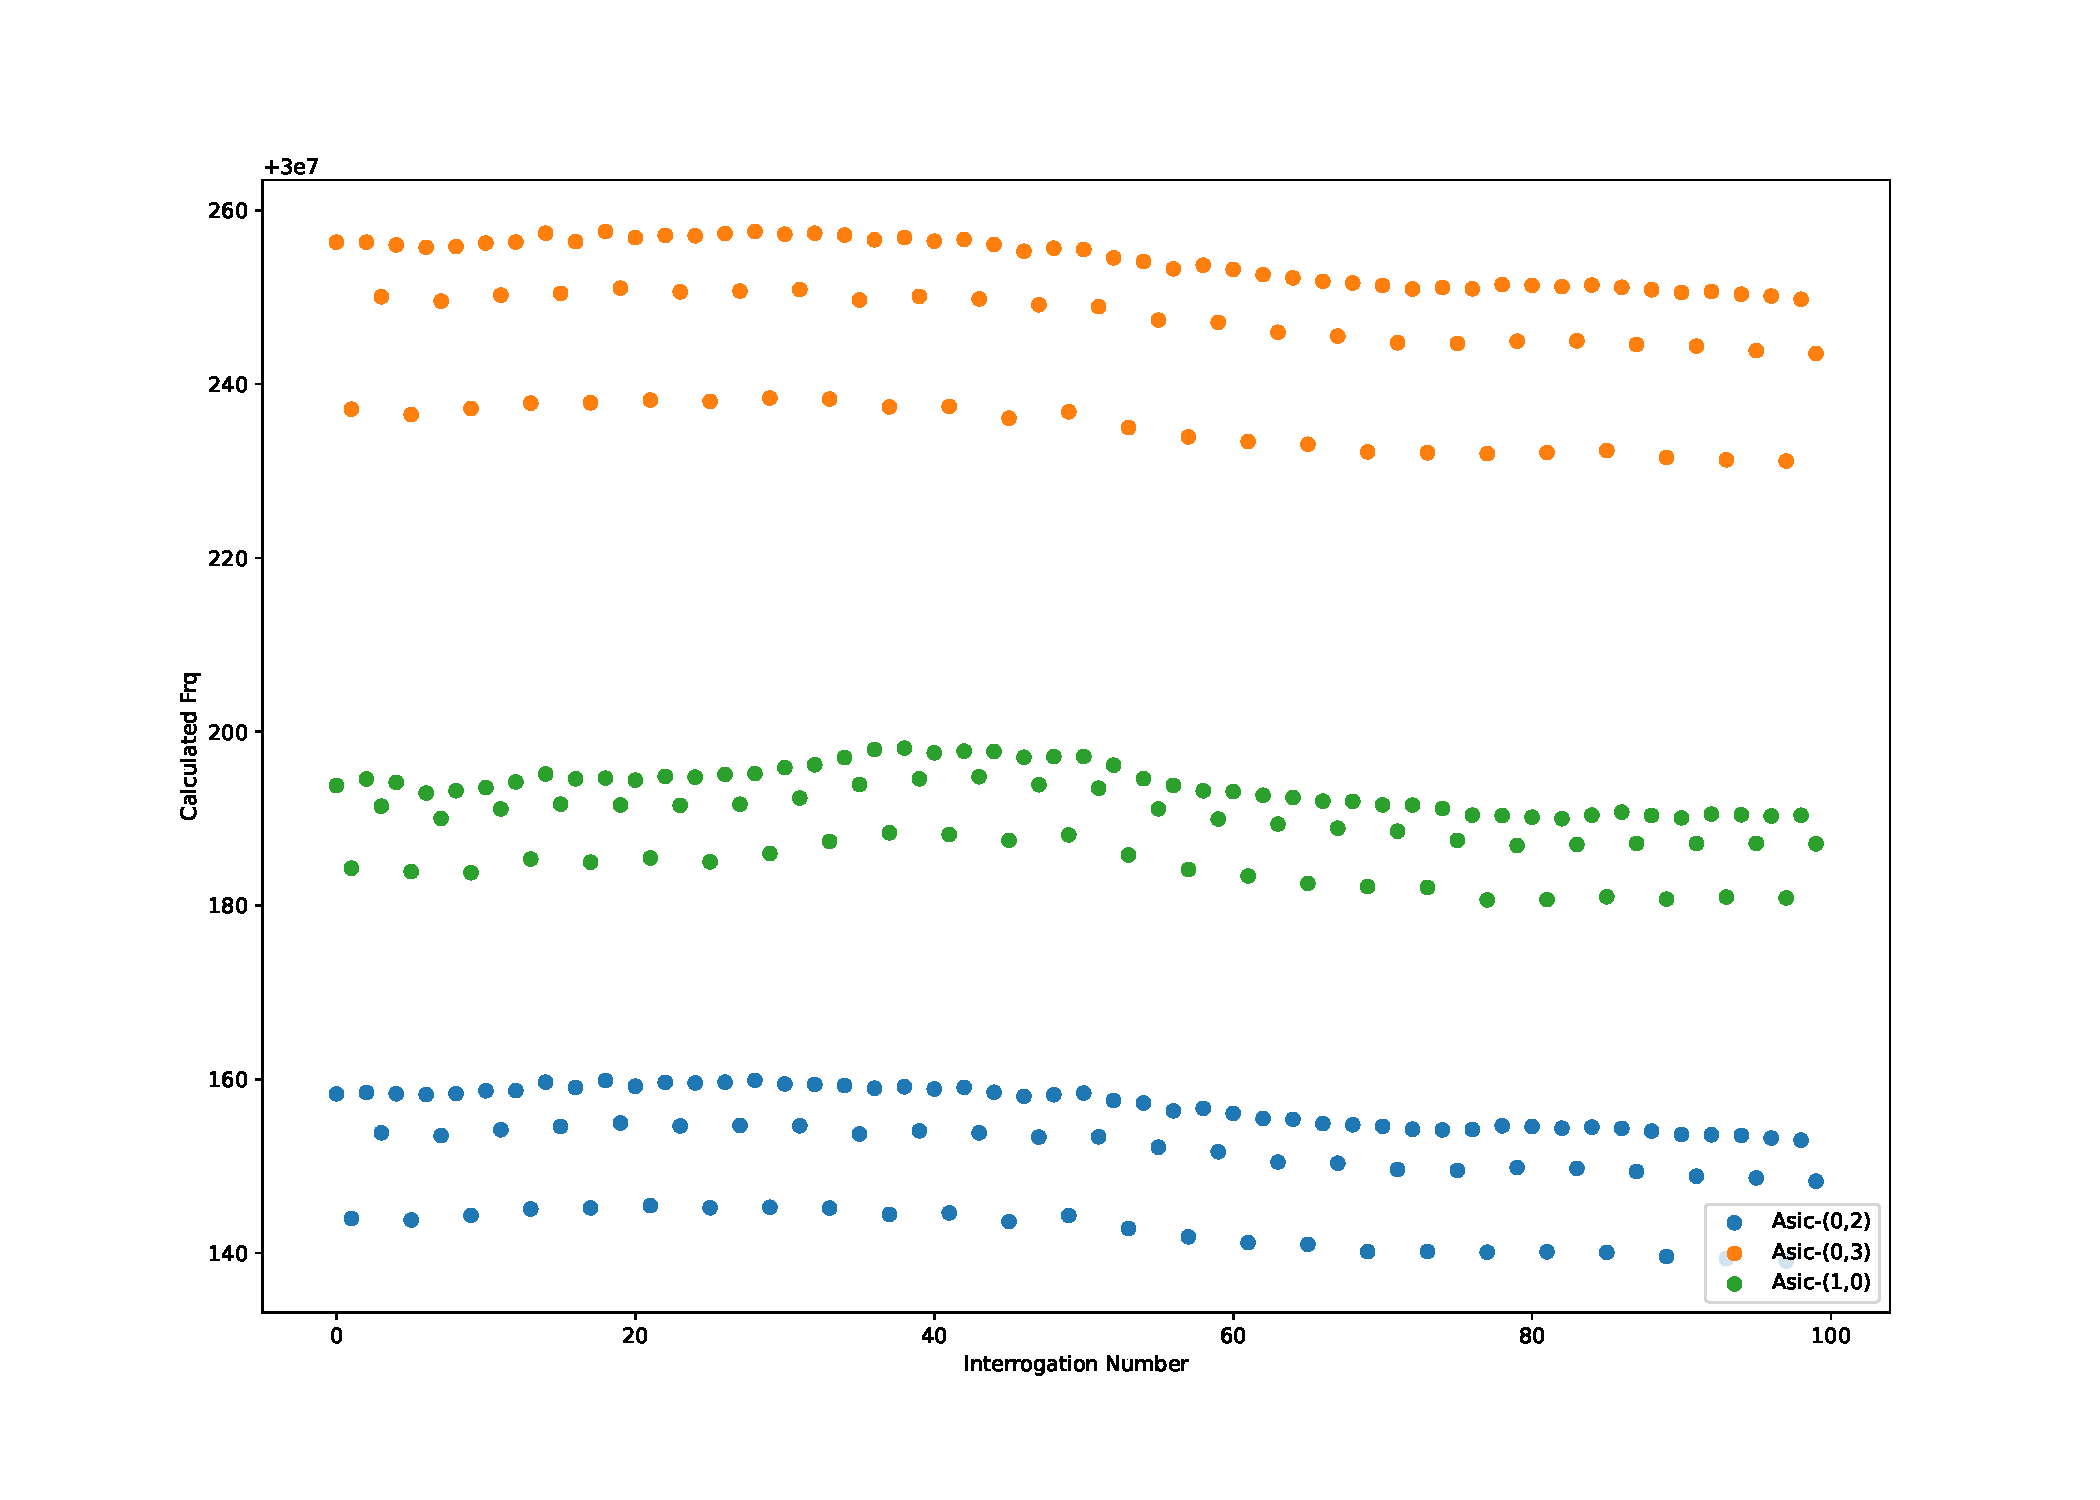
\includegraphics[width=0.5\textwidth]{images/slow_example.pdf}
\caption{}
\end{figure}






%% 0.1 Hz interrogation calibration 
\begin{table}
	\begin{center}
		\begin{tabular}{|c|c|c|c|}
			\hline
			FPGA Position & Mean (30~\unit{MHz}) & STD & $\frac{\delta f}{f_{o}}$*1e6 (ppm) \\
			\hline
			(0,0) & 243.223 & 3.895 & 0.130 \\
			\hline
			(0,1) & 187.225 & 4.631 & 0.154 \\
			\hline
			(0,2) & 151.020 & 6.255 & 0.208 \\
			\hline
			(0,3) & 246.553 & 8.229 & 0.274 \\
			\hline
			(1,0) & 188.851 & 4.521 & 0.151 \\
			\hline
			(1,1) & 207.837 & 6.468 & 0.216 \\
			\hline
			(1,2) & 111.344 & 7.882 & 0.263 \\
			\hline
			(1,3) & 156.660 & 9.985 & 0.333 \\
			\hline
			(2,0) & 348.263 & 6.748 & 0.225 \\
			\hline
			(2,1) & 190.976 & 8.622 & 0.287 \\
			\hline
			(2,2) & 196.369 & 9.919 & 0.331 \\
			\hline
			(2,3) & 148.284 & 11.844 & 0.395 \\
			\hline
			(3,0) & 179.718 & 8.375 & 0.279 \\
			\hline
			(3,1) & 207.859 & 10.655 & 0.355 \\
			\hline
			(3,2) & 188.123 & 11.836 & 0.395 \\
			\hline
			(3,3) & 165.011 & 13.725 & 0.457 \\
			\hline
		\end{tabular}
	\end{center}
	\caption{FPGA calibration results based on hard interrogations at a frequnecy of 0.1~\unit{Hz}.
	These data are more tightly clusted together due to the longer wait time between each interrogation, and are not easily separable as done in Table~\ref{tab:fpga_calibration}.
	The listed mean is the simple geometric mean and standard deviation for a one hour run time.
	}
	\label{tab:fpga_slow_calibration}
\end{table}


\subsection{Charge Auto-Calibration of each Pixel}~\label{sec:charge_calibration}

Natural decay products produced by $^{39}$Ar provide a continous source of incoming current across a LArTPC.

%% schematic of PCB

\section{Timing Stability}

We describe here the methods of measuring a stable time for different configurations of the nodes.
We also comment on the results of the timing with resepect to the minimum required timing sensitivity in order to have accurate timestamp reconstruction.

\section{Power and Current Characteristics}

There are test pads on the PCBs used to measure the voltage stability of the different FPGA voltages.
For each voltage, there is also a single 1~$\unit{\Omega}$ probe-resistor.
This resistor is used to measure the relative current drawn from each of the voltage sections on the PCB.

\section{Analysis of Systematics for Different System Implementations}

The essential features of the digital node in the Q-Pix readout are the properties of the local oscillator.
The frequency, relative phases, and stability of the oscillator determine the power consumption, packet transaction time, minimum timestamp resolution, which determines maximum current measurements, and affects packet loss probability in larger tile systems.
It is not an understatement to say that the successful development of the digital node relies on the development of the local oscillator.

\section{Towards the Integration of the Aggregator Node}

In the studies presented here, The aggregator node which was used was the Zybo Z7-20.


\section{Comments on A Super-DAQ-Node}

Each APA module within a larger DUNE module must ultimately be interconnected so that the entire module can be readout.
As described above, a single modular tile is controlled by an individual DAQ node, where many constitute a complete APA.
Therefore, we refer to the device that digitally multiplexes all of the DAQ node data as the "Super DAQ Node" (SDN).
Then, we imagine the final multiplexing stage for an entire DUNE module as an array of SDNs, each of which consistute an array of DAQ nodes, where each DAQ node is a 2-D array of Q-Pix based ASICs.

The total number of request SDNs within the full dune module depends on the final size of a DAQ-node controlled tile.

%% high level figure here from TPC -> Integrator -> Digital Node -> Aggregator -> SuperDAQ-Node -> WIC -> Disc

\section{The Back-End Summary}
